% Created 2020-05-06 mié 14:10
% Intended LaTeX compiler: pdflatex
\documentclass[a4paper, 12pt]{article}
\usepackage[utf8]{inputenc}
\usepackage[T1]{fontenc}
\usepackage{graphicx}
\usepackage{grffile}
\usepackage{longtable}
\usepackage{wrapfig}
\usepackage{rotating}
\usepackage[normalem]{ulem}
\usepackage{amsmath}
\usepackage{textcomp}
\usepackage{amssymb}
\usepackage{capt-of}
\usepackage{hyperref}
\usepackage{float, amsfonts, commath, mathtools, proba}
\author{Tabaré Pérez}
\date{\today}
\title{Lecture 16 - 2: Recap of Maximum Likelihood Estimation for Multinomial and Gaussian Models}
\hypersetup{
 pdfauthor={Tabaré Pérez},
 pdftitle={Lecture 16 - 2: Recap of Maximum Likelihood Estimation for Multinomial and Gaussian Models},
 pdfkeywords={},
 pdfsubject={},
 pdfcreator={Emacs 26.3 (Org mode 9.3.6)}, 
 pdflang={English}}
\begin{document}

\maketitle
\section*{Introduction}
\label{sec:org024e83c}

So far, in clustering we have assumed that the data has no probabilistic
generative model attached to it, and we have used various iterative algorithms
based on similarity measures to come up with a way to group similar data points
into clusters. In this lecture, we will assume an underlying probabilistic
generative model that will lead us to a natural clustering algorithm called the
E-M algorithm .

While a “hard" clustering algorithm like k-means or k-medoids can only provide a
cluster ID for each data point, the EM algorithm, along with the generative
model driving its equations, can provide the posterior probability (“soft"
assignments) that every data point belongs to any cluster.

The E-M algorithm will also form the basis for a portion of Project 4 in which we
explore collaborative filtering via Gaussian mixtures.

\section*{Video}
\label{sec:orge3d2a4d}

Today, we will talk about mixture model and the E-M algorithm. So first, let me
start by reminding you the types of distributions that you have already seen in
the class. What we will do today will kind of combine two of them. So the first
generative model that we've seen were \textbf{MULTINOMIALS}.

So in the case of multinomials, we assume that we have some set of possible
outcomes.

If we're talking about language, it will be maybe the vocabulary, capital
\(\mathcal{W}\), and we would also assume that we have certain likelihood to
generate particular word \(w\) in this vocabulary:

\begin{equation}
\label{eq:orgd717e3e}
\mathcal{W}; \prob(w|\theta) = \theta_w, \sum_{w \in \mathcal{W}} \theta_w = 1, \theta_w \geq 0
\end{equation}

So it means that the likelihood of generating \(w\), given
parameters \(\theta\) would be \(\theta_w\).

Another example that you can be thinking about is about a dice. Maybe our dice
is a normal dice and it will be 1 divided by 6 for every single edge of the
dice. So if it is some inappropriate dice, you would have different probability
for different sides.

And we know the sum of all these parameters because form probability
distribution have to be one, if we go over all the words in the vocabulary and
we also assume that each one of those \(\theta\)s is a non-negative number.

So now, we've said that given these multinomials, we can actually compute the
likelihood of a certain document. And since we're generating all the words in
the document independently of each other, we can just say:

\begin{equation}
\label{eq:org073fa52}
\prob(D|\theta) = \prod_{w \in \mathcal{W}} \theta_{w}^{n(w)}
\end{equation}

The likelihood of a document \(D\), which contains number words from \(w_1\) to
\(w_n\), given \(\theta\)s, would be just a product when we go through all the
words in our vocabulary. And then, we look how many times it would appear and we
would multiply \(\theta_w\) accordingly.

So if this will be the count of the words \(w\) in the document \(D\), then this
expression will give us the likelihood of the document, OK?

So this is one example of the distributions that we've seen. And then we've seen
a different distribution which were called \textbf{GAUSSIANS}.

So in this particular case, it's very easy for us to think about Gaussians in
terms of the geometric view:

\begin{figure}[H]
\centering
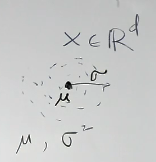
\includegraphics[width=0.2\textwidth]{./pic/u04-02-fig-01.png}
\caption{\label{fig:org171fb92}Geometric view of Gaussians}
\end{figure}

We assume that all all these different points and these points would have a
particular center, and they also would have variance and these are the two
parameters that will control our Gaussians.

I will establish where the points are kind of clustered together, and this is we
call it \(\mu\) is the center of the Gaussian.

And we will also have the variance for which we will use this notation,
\(\sigma^2\). And now, depending of how do you decide about the variance, we can
have all the points which are really close kind of collocated together, or they
may be farther spread around for large values of the variance. So in this
particular instance, we can actually look at the likelihood of certain points to
be generated by a given Gaussian, so given \(\mu\) and given variance:

\begin{equation}
\label{eq:orgc0188a1}
\prob(x|\mu, \sigma^2) 
\end{equation}

Again, we can look at one point and let's say we have several different
Gaussians, and it will have different probability depending on which of these
Gaussians we selected, which \(\mu\) and which \(\sigma^2\) we selected and in
this case, we will sometimes use slightly different notation, but the idea is
exactly the same:

\begin{equation}
\label{eq:org183a484}
\prob(x|\mu, \sigma^2) = \mathcal{N}(x; \mu, \sigma^2 I) = {\frac{1}{(2\pi\sigma^2)^{\frac{d}{2}}}} {e^\left( {-\frac{1}{2\sigma^2} \norm{x-\mu}^2} \right)} 
\end{equation}

And I remind you that \(d\) is just the size of our vector. Here, we are in 2D,
but typically we're going to be looking at much higher dimensions.

So here, it's actually very easy to see that the points which are farther
located from our center would have lower probabilities than points that are very
closely located to the center.

But what I want to tell you looking at these two distributions that what we've
done in the previous lecture, we actually answered a number of questions. And
we've seen, independently, which generative model we looked at. We kind of asked
similar questions and solved them using similar technique.

So the first question that we asked is: how I can actually estimate these
parameters? How do I know what are those \(\theta\)s, \(\theta_w\), in the case
of multinomial, or \(\mu\) and \(\sigma^2\) in the case of Gaussian?

And the criteria that we used was the maximum likelihood estimator (MLE) . So we
estimated parameter using MLE, Maximum Likelihood Estimator, and what we've said
that given some particular document \(D\), we are looking for the values of
these parameters that are going to give the highest likelihood to our observed
data.

And if you remember, we took our usual tricks. We took the derivative with
respect to parameters, made them equal to \(0\), and demonstrated how these
parameters would look like.

And we did the same, both for multinomials and for Gaussians and not
surprisingly, what we've got is very consistent with our intuition.

For instance, in the case of Gaussians, we demonstrated that the estimated
\(mu\) for our Gaussian would be:

\begin{equation}
\label{eq:org0956bec}
\hat{\mu} = \frac{1}{n} \sum_{i=1}^{n} x^{(i)}
\end{equation}

Just a mean of all the points.

And similarly, we also demonstrated, using exactly the same technique, that if
we're estimating our \(\sigma^2\):

\begin{equation}
\label{eq:org77fbb73}
\hat{\sigma}^2 = \frac{1}{nd} \sum_{i=1}^{n} \norm{x^{(i)} - \mu}^2
\end{equation}

So this is the estimate that we are going to get if, again, we take the
corresponding expression, take the derivative, and that's what you did in your
exercises, and you will get this expression.
\end{document}